\subsection{Properties of the TTF Return Series}\label{sec:properties-ttf}
The daily log returns over the full sample are shown in Fig.~\ref{fig:ttf-log-returns}. The three data splits of Sec.~\ref{sec:data-split} are marked.

\begin{figure}[htbp]
    \centering
    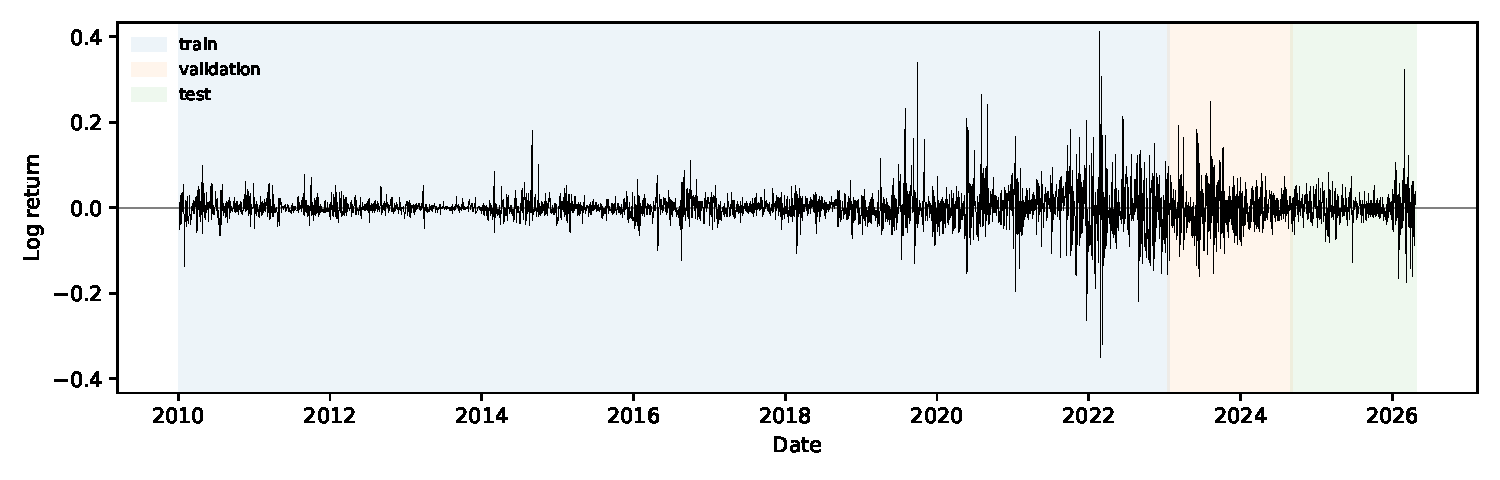
\includegraphics[width=\textwidth]{figures/ttf_log_returns.pdf}
    \caption{Daily TTF log returns with the train, validation and test splits}
    \label{fig:ttf-log-returns}
\end{figure}

Table~\ref{tab:ttf-stats} reports the distributional properties of the TTF return series, full sample and per data split. These statistics are the reference values against which generated returns are compared in the following sections. 

\begin{table}[htbp]
\centering
\begin{tabular}{lrrrr}
\toprule
 & Full & Train & Validation & Test \\
\midrule
$n$                    & 3{,}997  & 3{,}197  & 399      & 401    \\
Mean                   &  0.0003  &  0.0005  & $-$0.0014 &  0.0006  \\
Standard deviation     &  0.0395  &  0.0377  &  0.0515  &  0.0401  \\
Skewness               &  0.70    &  0.71    &  0.59    &  0.91    \\
Excess kurtosis        & 14.91    & 19.08    &  2.53    & 13.24    \\
Minimum                & $-$0.3524 & $-$0.3524 & $-$0.1615 & $-$0.1749 \\
Maximum                &  0.4128  &  0.4128  &  0.2483  &  0.3229  \\
$1\%$ quantile         & $-$0.1153 & $-$0.1129 & $-$0.1248 & $-$0.1291 \\
$99\%$ quantile        &  0.1239  &  0.1224  &  0.1639  &  0.0885  \\
$P(|x| > 0.05)$        &  0.117   &  0.099   &  0.253   &  0.130   \\
$P(|x| > 0.10)$        &  0.030   &  0.027   &  0.058   &  0.025   \\
\midrule
$C(1)$                 &  0.033   &  0.067   & $-$0.096 &  0.008   \\
$C_2(1)$               &  0.364   &  0.392   &  0.128   &  0.288   \\
$C_2(2)$               &  0.280   &  0.310   &  0.206   &  0.061   \\
$C_2(5)$               &  0.215   &  0.236   &  0.105   &  0.094   \\
$C_2(10)$              &  0.112   &  0.117   &  0.148   &  0.011   \\
\bottomrule
\end{tabular}
\caption{Distributional statistics and autocorrelation of daily TTF log returns, full sample and per data split}
\label{tab:ttf-stats}
\end{table}

\textbf{Heavy tails.} The excess kurtosis of the full series is \num{14.91}, compared to 0 for a normal distribution (Sec.~\ref{sec:stylized-facts}). Absolute returns exceed \SI{10}{\percent} on \SI{3}{\percent} of trading days. The heavy tails are not distributed evenly across the data splits. The training split, which contains the 2021 to 2022 crisis, has an excess kurtosis of \num{19.08}. The test split, which contains the 2026 disruption, has \num{13.24}. Both episodes are described in Sec.~\ref{sec:gas-markets}. The validation split does not contain a comparable event and has an excess kurtosis of \num{2.53}.

\textbf{Asymmetry.} The skewness of the full series is \num{0.70}, indicating that large positive returns are more likely than large negative returns (Sec.~\ref{sec:stylized-facts}). The skewness is positive for all data splits, with the training split at \num{0.71}, the validation split at \num{0.59} and the test split at \num{0.91}. As reported in Sec.~\ref{sec:m1-construction}, the transition days account for most of the positive skew. Skewness falls to \num{0.26}
when transition days are excluded. The remaining asymmetry is consistent with the supply disruptions described in
Sec.~\ref{sec:gas-markets}. Such events raise prices sharply, while no comparable mechanism lowers them. The positive skew is consistent with the right-skewed volatility smile reported for energy markets in Sec.~\ref{sec:implied-vol}.

\textbf{Volatility clustering.} The autocorrelation of returns at $\tau=1$, Eq.~\eqref{eq:autocorrelation}, is \num{0.033} and stays close to 0 across all data splits. The autocorrelation of squared returns, Eq.~\eqref{eq:vol-clustering}, is \num{0.364} at $\tau=1$, and decays slowly, to \num{0.280} at $\tau=2$, \num{0.215} at $\tau=5$ and \num{0.112} at $\tau=10$. The slow decay is the volatility clustering described in Sec.~\ref{sec:stylized-facts}.
The training split decays smoothly as well, while the validation and
test splits do not.
In the validation split the autocorrelation rises from \num{0.128} at $\tau=1$ to \num{0.206} at $\tau=2$, falls to \num{0.105} at $\tau=5$ and rises again to \num{0.148} at $\tau=10$. In the test split it drops from \num{0.288} to \num{0.061} between $\tau=1$ and $\tau=2$, rises to \num{0.094} at $\tau=5$ and falls to \num{0.011} at $\tau=10$. The training split holds \num{3197} of the \num{3997} observations, so the decay of the full sample follows from the training split.

The heavy tails and the volatility clustering of the test split originate in the 2026 disruption described in Sec.~\ref{sec:gas-markets}. The test split is further examined with that period removed. Table~\ref{tab:test-spike} reports the distributional properties of the full test split and the test split excluding the period from 2026-02-01 to 2026-04-30. The excluded period covers \num{57} of the \num{401} trading days.


\begin{table}[htbp]
\centering
\begin{tabular}{lrr}
\toprule
 & Test & Test excluding 2026 disruption \\
\midrule
$n$                & 401     & 344 \\
Standard deviation &  0.0401 &  0.0288 \\
Skewness           &  0.91   & $-$0.06 \\
Excess kurtosis    & 13.24   &  1.57 \\
$P(|x| > 0.10)$    &  0.025  &  0.006 \\
$C_2(1)$           &  0.288  &  0.042 \\
\bottomrule
\end{tabular}
\caption{Test split statistics with and without the 2026 disruption}
\label{tab:test-spike}
\end{table}
When the 2026 disruption is excluded, the test split does not show heavy tails, asymmetry or volatility clustering. The validation split has the highest standard deviation of all splits, and contains no comparable single event. The returns of the validation split are uniformly large, while the returns of the test split are moderate outside a single episode. 
The tails of the return distribution determine the value of out-of-the-money options (Sec.~\ref{sec:stylized-facts}). 
The excess kurtosis is \num{13.24} in the test split and \num{2.53} in the validation split. For this reason, the generated returns are compared with the test split in the following sections. The model selection of Sec.~\ref{sec:model-selection} is based on it as well. The consequence of this choice is discussed in Sec.~\ref{sec:limitations}.